\chapter{Forward pixel maintenance during LS1\label{sec:fpixls1}}

As mentioned in Section~\ref{sec:matbudg-pilot}, the CMS pixel detector was extracted from the experimental cavern and housed in a special facility aboveground for repairs, maintenance, and calibration during the first long shutdown (LS1) of the LHC from February 2013 to February 2015.

Starting in the summer of 2012 until the extraction of the pixel detector in May 2013, I worked with the UC Davis forward pixel team to set up the lab that would be used to house the extracted pixel detector. Each of the four half-cylinders of the forward pixel (FPIX) detector and two half-barrels of the barrel pixel (BPIX) detector was stored in a protective insulated box called a ``cold box", with temperature and humidity controlled by the following systems:

\begin{itemize}
\item \textbf{Water-glycol cooling system:} A system of pipes cycles a chilled 50\%/50\% mixture by volume of water and glycol continuously through the cooling tubes of the pixel half-cylinder supply tube. The water-glycol chiller set point is 0$^{\circ}$ C for the BPIX cold boxes and -2$^{\circ}$ C for the FPIX cold boxes; these set points have been empirically optimized so as to achieve a temperature below 10$^{\circ}$ C within the cold boxes, as monitored by temperature sensors at various positions in the boxes. The purpose of keeping the general environment of the pixel detector cold is to minimize the spread of radiation-induced defects in the crystal structure of the silicon sensors due to thermal agitation.
\item \textbf{C$_{6}$F$_{14}$ cooling system:} A system of pipes cycles chilled liquid C$_{6}$F$_{14}$ through the cooling tubes that serve the sensitive regions of the pixel-half cylinder (panels in FPIX and modules in BPIX). The C$_{6}$F$_{14}$ is kept at a controlled temperature by a dedicated C$_{6}$F$_{14}$ chiller. When the panels or modules of the half-cylinder are turned on for testing and maintenance, extra heating occurs due to the currents in the electronics; thus, the C$_{6}$F$_{14}$ cooling system serves to counter this extra heating and keep the temperature at the panels or modules below 20$^{\circ}$ C. The C$_{6}$F$_{14}$ cooling system, with the chiller set point set to -15$^{\circ}$ C, is only used when the half-cylinder panels or modules are powered on.
\item \textbf{Dry air system:} To prevent humidity from damaging the sensitive electronics of the pixel detector, the interior of the cold box is supplied with room-temperature dry air from an air dryer via pipe lines leading into the boxes, while the humidity inside the boxes is monitored by dew point sensors at various positions.
\end{itemize}

I helped to prepare the cold boxes for transport to the lab and to set up all three of the above-listed systems to serve the cold boxes, as well as the power supply crates and DAQ systems to power and read-out respectively the forward pixel detector half-cylinders. Once the pixel detector was extracted and the half-cylinders and half-barrels were successfully installed in their respective cold boxes, the forward pixel team proceeded to tackle known longstanding problems with certain panels in the FPIX. Here is a brief list of the issues:

\begin{itemize}
\item \textbf{Slow channels:} the analog signal from certain panels has a slow rise time, resulting in lost bandwidth.
\item \textbf{A panel with one dead ROC:} this problem is insignificant and not worth the delicate operation of replacing the panel, so it was left alone.
\end{itemize}

Many of these problems were traced to misaligned or dislodged cables that provide communication from the portcards to the panels, for various functions such as programming the ROCs and reading out analog signals. I participated in the diagnosis of these problems by assisting in reading out the analog signal coming from problematic panels at different points along the readout circuit, and by replacing malfunctioning portcards.

After all the repairs had been performed, including the replacement of certain panels, the FPIX calibration sequence was performed on each half-cylinder individually. This set of calibration procedures programs and optimizes the various parameters of the FPIX readout system (illustrated schematically in Figure~\ref{fig:cms-pixel-readout}); a treatment of these calibration procedures is beyond the scope of this dissertation, but a detailed description can be found in this source~\cite{CMS-pixel-calibrations}.

\begin{figure}[hbtp]
  \begin{center}
    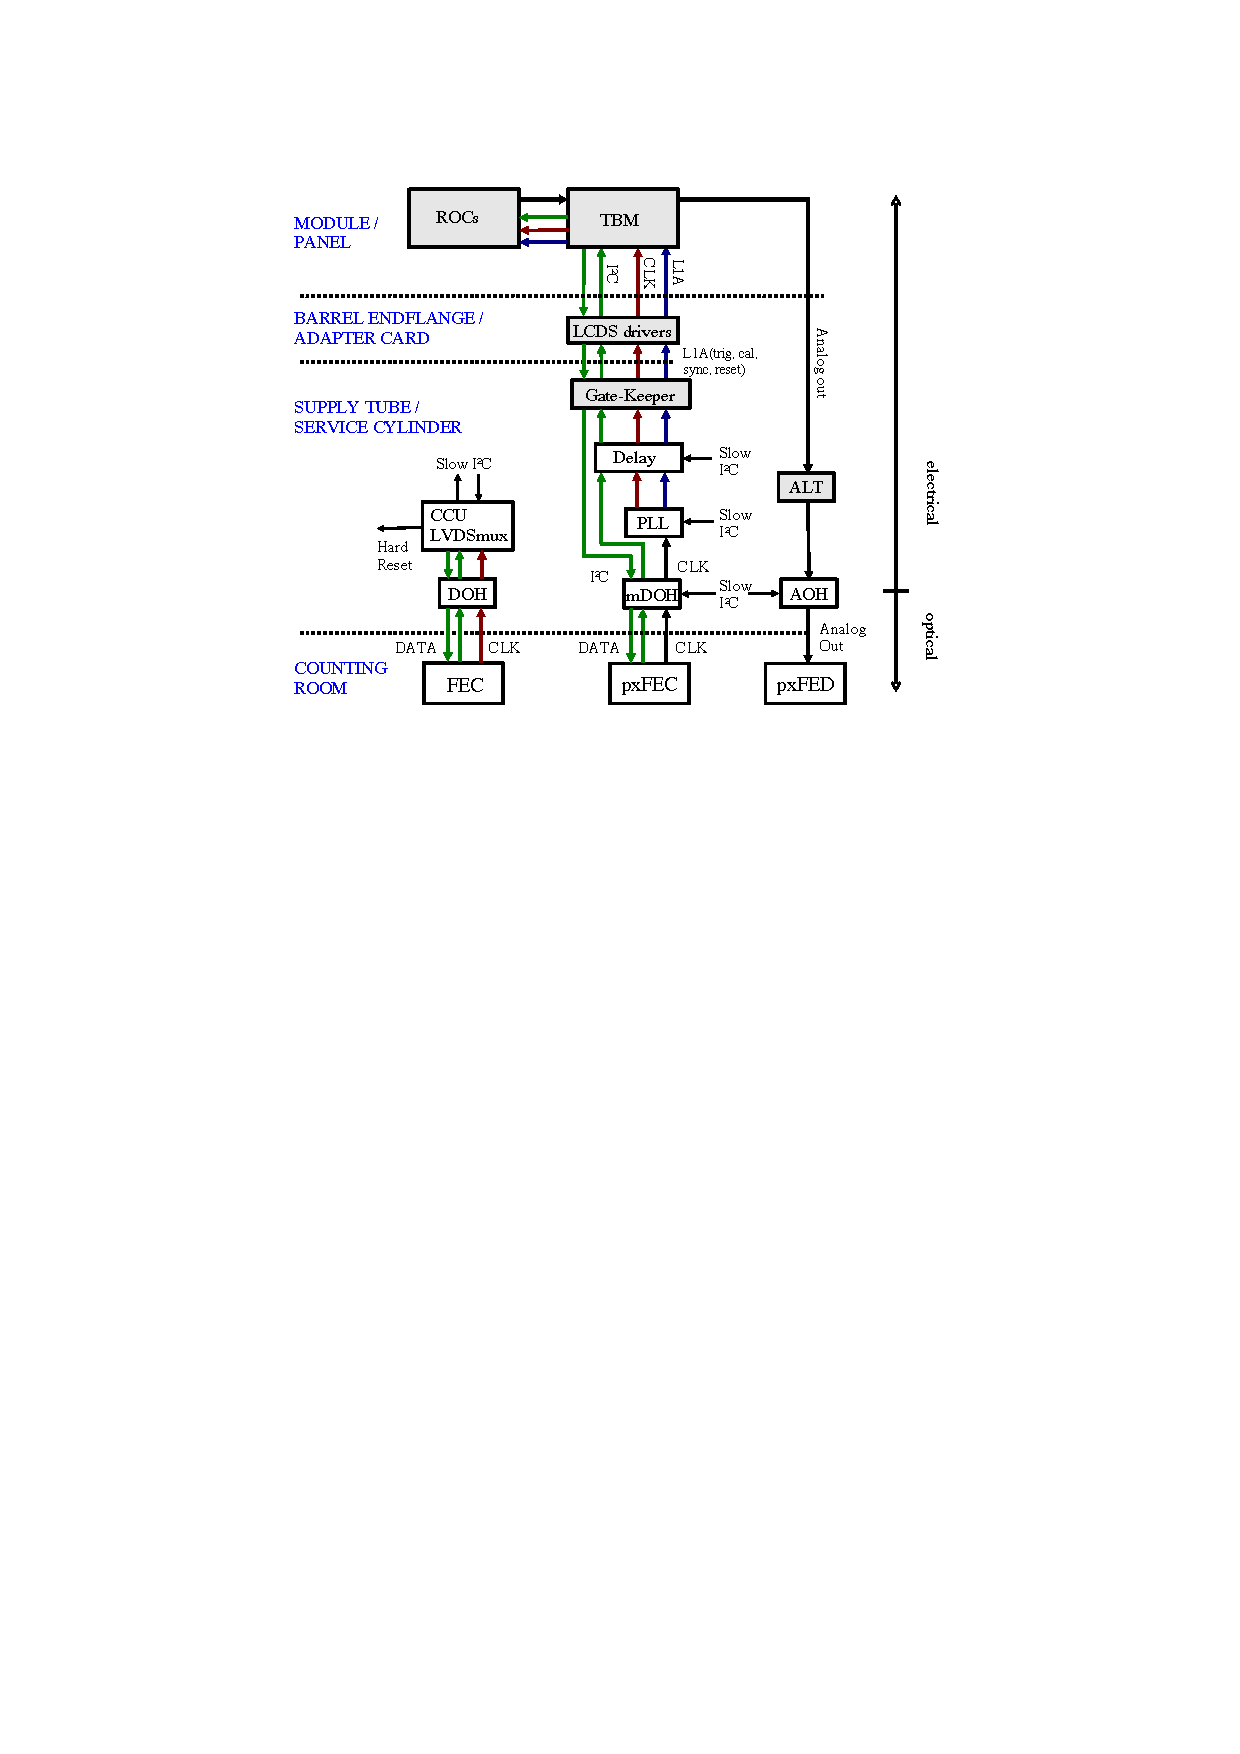
\includegraphics[width=2.0\cmsFigWidth]{figures/cms-pixel-readout}
    \caption{Diagram of the CMS pixel control and readout system. ~\cite{1748-0221-3-08-S08004}}
    \label{fig:cms-pixel-readout}
  \end{center}
\end{figure}

All four FPIX half-cylinders were successfully calibrated in the lab; I participated in the calibration of three out of the four. After the pixel detector was reinstalled in the experimental cavern at the end of 2014, I assisted the forward pixel team in calibrating the FPIX once more (this time calibrating all half-cylinders simultaneously instead of separately) to prepare it for data-taking at the new proton-proton collision energy of 13 TeV.